\documentclass[xcolor={dvipsnames}]{beamer}

\usepackage[T1]{fontenc}

\usepackage{amssymb}
\usepackage{stmaryrd}
\usepackage{amsfonts}
\usepackage{amsmath}
\usepackage{latexsym}
\usepackage{url}

\usepackage{listings}

\usepackage{mathtools}
\usepackage{calc}
\usepackage{lmodern}
\usepackage{changepage}
\usepackage{hyperref}
\usepackage{graphicx}

\usetheme{Madrid}

\setbeamertemplate{caption}{\raggedright\insertcaption\par}

\title{Adding Types and Theory Kinds to Drasil}
\author[J. Balaci]{Jason Balaci\\\small{}Under the supervision of Dr. Jacques Carette}

\institute[McMaster U.]{McMaster University}
\date{Dec. $8^{\text{th}}$, 2022}

\AtBeginSection[]
{
  \begin{frame}
    \frametitle{Table of Contents}
    \tableofcontents[currentsection]
  \end{frame}
}

% For code highlighting
\usepackage[newfloat,outputdir=build]{minted}
\usemintedstyle{colorful}

% For loading images
\usepackage{graphicx}
\graphicspath{ {./assets/img/} }


% For fancy pictures
\usepackage{tikz}
\usetikzlibrary{shapes,arrows,cd}
\usetikzlibrary{babel} % Make sure quiver/tikz uses babel
\usetikzlibrary {arrows.meta,graphs,graphdrawing}
\usegdlibrary {layered}

\usepackage{todonotes}

\usepackage{svg}

\newcommand{\inlineHs}[1]{\mintinline{haskell}|#1|}
% Command based on: https://tex.stackexchange.com/questions/266811/define-a-new-command-with-parameters-inside-newcommand
\newcommand{\codeName}[1]{\expandafter\newcommand\csname #1\endcsname{\inlineHs{#1}}}

\codeName{CodeExpr}
\codeName{Expr}
\codeName{ModelExpr}

\begin{document}

%------------------------------------------------------------------------------
% TITLE
%------------------------------------------------------------------------------
\frame{\titlepage}

%------------------------------------------------------------------------------
% TABLE OF CONTENTS
%------------------------------------------------------------------------------

\begin{frame}
\frametitle{Table of Contents}
\tableofcontents
\end{frame}

%------------------------------------------------------------------------------
% OVERVIEW
%------------------------------------------------------------------------------
\section{Overview}

\begin{frame}
  \frametitle{Overview}

  \begin{enumerate}
    \item Background: Drasil
    \item 4 Research Areas:
      \begin{enumerate}
        \item Structuring theories
        \item Restricting mathematical expression terminology to appropriate
              contexts
        \item Well-typedness of mathematical expressions
        \item An extensible database for remembering everything
      \end{enumerate}
  \end{enumerate}

\end{frame}

%------------------------------------------------------------------------------
% BACKGROUND: DRASIL
%------------------------------------------------------------------------------
\section{Drasil}

\begin{frame}
  \frametitle{What is Drasil? How does it work?}
  \framesubtitle{\textquotedblleft{}Generate All The Things!\textquotedblright{}}

  \begin{columns}
    \begin{column}{0.45\textwidth}
      
\includegraphics[width=\textwidth]{drasil_logo.png}
    \end{column}
    \hfill
    \begin{column}{0.45\textwidth}
      \begin{enumerate}
        \item Software generation suite for ``well-understood'' domains
        \item De-duplicating and capturing knowledge across software artifacts
        \item Uses a Software Requirements Specification (SRS) template to
              decompose scientific problems and generate software
      \end{enumerate}
    \end{column}
  \end{columns}

\end{frame}

\begin{frame}
  \frametitle{Example}
  \framesubtitle{SRS to Code}

  \begin{columns}
    \begin{column}{0.45\textwidth}
      Using SRS components:
      \begin{enumerate}
        \item Symbols (inputs, outputs, and everything in-between)
        \item Problem description and goals
        \item Assumptions
        \item Abstract theories
        \item Concrete theories
        \item \(\ldots{}\)
      \end{enumerate}
    \end{column}
    \hfill
    \begin{column}{0.5\textwidth}
      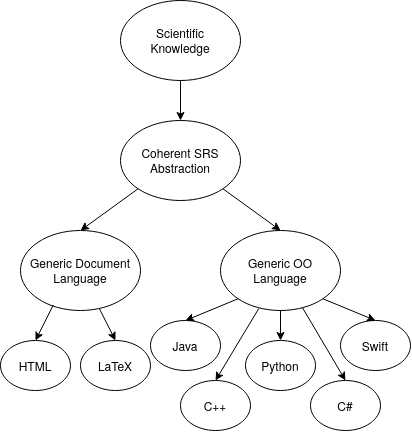
\includegraphics[width=\textwidth]{roughNetworkOfDomains.png}
    \end{column}
  \end{columns}

\end{frame}

%------------------------------------------------------------------------------
% THEORIES
%------------------------------------------------------------------------------
\section{Theories in Drasil}

\begin{frame}[fragile]
  \frametitle{How are theories used?}
  
  \begin{columns}
    \begin{column}{0.4\textwidth}
      \begin{center}
        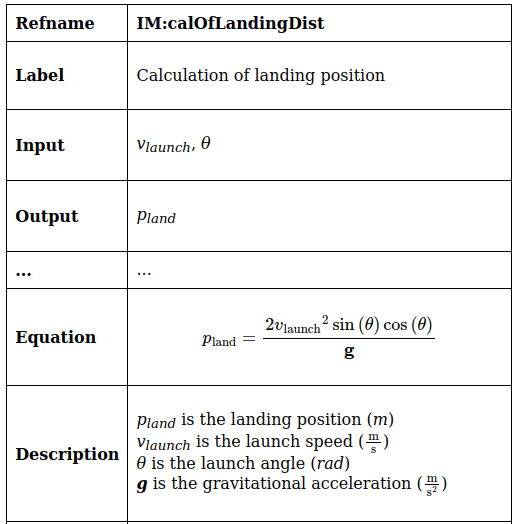
\includegraphics[width=0.9\textwidth]{concreteTheory.png}
      \end{center}
    \end{column}
    \hfill
    \begin{column}{0.575\textwidth}
\begin{minted}[fontsize=\scriptsize,breaklines]{haskell}
...
landPosExpr :: Expr
landPosExpr = sy landPos $= 2 * square (sy launSpeed) * sin (sy launAngle) * cos (sy launAngle) / sy gravitationalAccelConst

landPosRC :: RelationConcept
landPosRC = makeRC "landPosRC" (nounPhraseSP "calculation of landing position") landPosConsNote landPosExpr
...
\end{minted}
    \end{column}
  \end{columns}
\end{frame}

\begin{frame}[fragile]
  \frametitle{How are theories used?}

\begin{minted}[breaklines,frame=single,framesep=5pt,rulecolor=lightgray,fontsize=\scriptsize]{haskell}
relToQD :: ExprRelat c => ChunkDB -> c -> QDefinition
relToQD sm r = convertRel sm (r ^. relat)

convertRel :: ChunkDB -> Expr -> QDefinition
convertRel d (BinaryOp Eq (C x) r) = ec (symbResolve d x) r
convertRel _ _ = error "Conversion failed"
\end{minted}

\vspace{2em}

\begin{minted}[breaklines,frame=single,framesep=5pt,rulecolor=lightgray,fontsize=\scriptsize]{java}
public static double func_p_land(double v_launch, double theta, double g_vect) {
  return 2 * Math.pow(v_launch, 2) * Math.sin(theta) * Math.cos(theta) / g_vect;
}
\end{minted}

\end{frame}

\begin{frame}[fragile]
  \frametitle{Decompose, classify, and encode}

\begin{minted}{haskell}
data ModelKinds e where
  NewDEModel            :: DifferentialModel -> ModelKinds e
  DEModel               :: RelationConcept   -> ModelKinds e
  EquationalConstraints :: ConstraintSet e   -> ModelKinds e
  EquationalModel       :: QDefinition e     -> ModelKinds e
  EquationalRealm       :: MultiDefn e       -> ModelKinds e
  OthModel              :: RelationConcept   -> ModelKinds e
\end{minted}

  \vspace{0.2cm}

  \begin{itemize}
    \item EquationalModel: \(x := f(x,y,z,\ldots{})\)
    \item EquationalConstraints: \(a \land b \land c \land \ldots{}\)
    \item EquationalRealm: \(x := f(x,y,z,\ldots{}) \lor x := g(x,y,z,\ldots{}) \lor \ldots{}\)
    \item DEModel \& NewDEModel: \(dy = f(x, y, \ldots{})\)
    \item OthModel: ?
  \end{itemize}
\end{frame}

\begin{frame}
  \frametitle{Ripple effects}

  \begin{itemize}
    \item Tangible categorization through type information.
    \item Structured creation, interaction, and analysis.
    \item Flexible, more opportunity for (domain-specific) interpretation.
      \begin{itemize}
        \item Specifically, opening up more opportunities for code generation.
      \end{itemize}
  \end{itemize}

\end{frame}

%------------------------------------------------------------------------------
% EXPRESSIONS
%------------------------------------------------------------------------------
\section{Expressions}

\begin{frame}[fragile]
  \frametitle{What are they used for?}

  In encoding\ldots{}
  \begin{columns}
    \begin{column}{0.3\textwidth}
      \begin{center}
        Code (OO)

        \vspace{1em}

\begin{minted}[breaklines,fontsize=\scriptsize]{python}
def theta(...):
  return math.asin(d * g / (v ** 2)) / 2
\end{minted}
      \end{center}
    \end{column}
    \hfill
    \begin{column}{0.3\textwidth}
      \begin{center}
        Concrete theories
        
        \vspace{1.4em}

        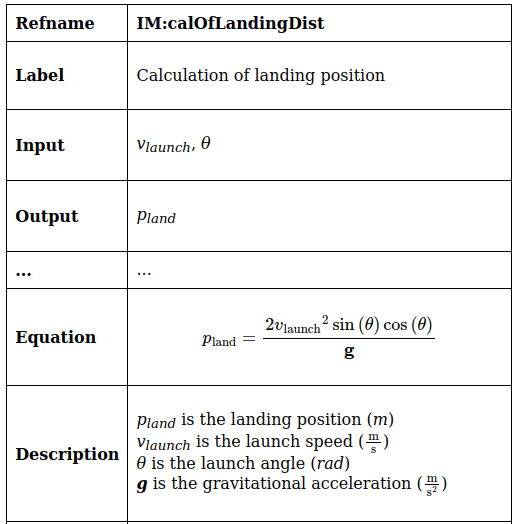
\includegraphics[width=\textwidth]{concreteTheory.png}
      \end{center}
    \end{column}
    \hfill
    \begin{column}{0.3\textwidth}
      \begin{center}
        Abstract theories
        
        \vspace{1em}

        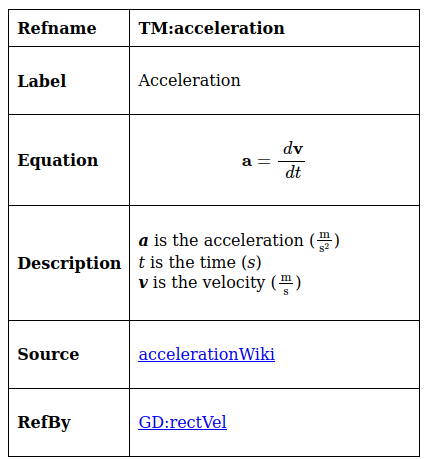
\includegraphics[width=\textwidth]{abstractTheory.png}
      \end{center}
    \end{column}
  \end{columns}
\end{frame}

\begin{frame}
  \frametitle{Restricting terms by context}

  \begin{enumerate}
    \item Split up the expression language by context
    \item Use a ``Typed-Tagless'' encoding to make usage seamless and
          interoperable
  \end{enumerate}

  \[\Expr{} \Rightarrow{} \Expr{} \cup{} \ModelExpr{} \cup{} \CodeExpr{}\]

\end{frame}

\begin{frame}
  \frametitle{Ripple effects}

  \begin{enumerate}
    \item Restricting terms by context
    \item Stop users from entering in un-translatable expressions
    \item Know when Equational Models are usable for code generation
  \end{enumerate}

\end{frame}

\begin{frame}[fragile]
  \frametitle{Validity of Expressions}

\begin{minted}[frame=single,framesep=5pt,rulecolor=lightgray]{haskell}
data Expr where
  Lit      :: Literal -> Expr
  AssocA   :: AssocArithOper -> [Expr] -> Expr
  AssocB   :: AssocBoolOper  -> [Expr] -> Expr
  C        :: UID -> Expr
  ...
\end{minted}

\begin{columns}
  \begin{column}{0.575\textwidth}
    \begin{minted}[frame=single,framesep=5pt,rulecolor=lightgray]{haskell}
illTyped :: Expr
illTyped = int 1 $+ str "Drasil"
    \end{minted}
    \vspace{0.5em}
    \begin{minted}[frame=single,framesep=5pt,rulecolor=lightgray]{java}
public static double func_ex() {
    return 1 + "Drasil";
}
    \end{minted}
  \end{column}
  \hfill
  \begin{column}{0.375\textwidth}
    \begin{minted}[frame=single,framesep=5pt,rulecolor=lightgray,breaklines]{console}
error: incompatible types: String cannot be converted to double
  return 1 + "Drasil";
           ^
    \end{minted}
  \end{column}
\end{columns}

\end{frame}

\begin{frame}
  \frametitle{Typing}

  \begin{enumerate}
    \item Adding \emph{bidirectional} type-checking.
    \item Type-checking and reporting en masse.
  \end{enumerate}

  \begin{columns}
    \begin{column}{0.475\textwidth}
      \begin{center}
        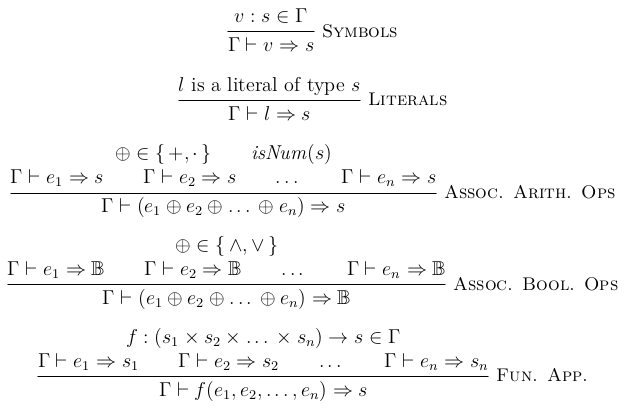
\includegraphics[width=\textwidth]{typeRulesLeft.png}
        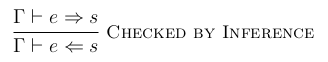
\includegraphics[width=0.55\textwidth]{typeRulesCheckByInfer.png}
      \end{center}
    \end{column}
    \hfill
    \begin{column}{0.475\textwidth}
      \begin{center}
        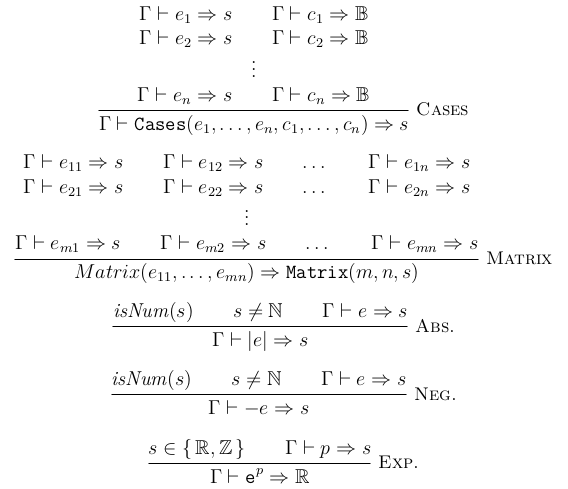
\includegraphics[width=\textwidth]{typeRulesRight.png}
      \end{center}
    \end{column}
  \end{columns}

  \vfill
  {\tiny \hfill \emph{Note: not all type rules shown here.}}
\end{frame}

\begin{frame}
  \frametitle{Ripple effects}

  \begin{enumerate}
    \item Found many typing issues and areas of code (e.g., vectors) that need
          more work
    \item First capture of implicit ``chunk'' constraints
    \item Realized we can move more ``checks'' to be done post-facto or
          on-demand
  \end{enumerate}

\end{frame}

%------------------------------------------------------------------------------
% DATA (CHUNKS)
%------------------------------------------------------------------------------
\section{Data in Drasil (\textquotedblleft{}Chunks\textquotedblright{})}

\begin{frame}
  \frametitle{How is data stored in Drasil?}

  \centering
  \includesvg[width=0.8\textwidth]{assets/img/chunksGoingIntoDrasil.svg}

\end{frame}

\begin{frame}[fragile]
  \frametitle{How is data stored in Drasil?}

\begin{minted}{haskell}
data ChunkDB = CDB 
  { symbolTable :: SymbolMap
  , termTable :: TermMap 
  , defTable  :: ConceptMap
  , _unitTable :: UnitMap
  , _traceTable :: TraceMap
  , _refbyTable :: RefbyMap
  , _dataDefnTable  :: DatadefnMap
  , _insmodelTable   :: InsModelMap
  , _gendefTable   :: GendefMap
  , _theoryModelTable :: TheoryModelMap
  , _conceptinsTable :: ConceptInstanceMap
  , _sectionTable :: SectionMap
  , _labelledcontentTable :: LabelledContentMap
  } --TODO: Expand and add more databases
\end{minted}

\end{frame}

\begin{frame}[fragile]
  \frametitle{Scaling against new \textit{kinds} of data}

  \begin{center}
    Mask the type information!
  \end{center}

\begin{minted}{haskell}
{-# LANGUAGE ExistentialQuantification, ConstraintKinds #-}

type IsChunk a = (HasUID a, HasChunkRefs a, Typeable a)

data Chunk = forall a. IsChunk a => Chunk a

type ChunkDB = Map UID Chunk

unChunk :: Typeable a => Chunk -> Maybe a
unChunk (Chunk c) = cast c
\end{minted}
\end{frame}

\begin{frame}[fragile]
  \frametitle{Scaling against new \textit{kinds} of data}
  \framesubtitle{Extra machinery}

\begin{minted}{haskell}
type ReferredBy = [UID]

type ChunkByUID = M.Map UID (Chunk, ReferredBy)

type ChunksByTypeRep = M.Map TypeRep [Chunk]

newtype ChunkDB = ChunkDB (ChunkByUID, ChunksByTypeRep)
\end{minted}
\end{frame}

\begin{frame}
  \frametitle{Ripple effects}

  \begin{enumerate}
    \item Everything is in one place!
    \item Chunk analysis capabilities:
      \begin{enumerate}
        \item (easier) type usage analytics
        \item chunk dependency tree
        \item find cyclic knowledge
        \item dumping all chunks at once
      \end{enumerate}
    \item ChunkDB arithmetic?
    \item (easier) Generalized chunk constraints!
    \item Usable ``base'' across Drasil-like projects
  \end{enumerate}
\end{frame}

%------------------------------------------------------------------------------
% FUTURE WORK
%------------------------------------------------------------------------------
\section{Future Work}

\begin{frame}
  \frametitle{Future Work}

  Regarding\ldots{}
  \begin{enumerate}
    \item Theories:
      \begin{enumerate}
        \item Explore alternative \inlineHs{ModelKinds} design.
        \item Explore remaining theories (e.g., structure \inlineHs{OthModel}s).
      \end{enumerate}
    \item Expressions:
      \begin{enumerate}
        \item Add (optional) typing to \inlineHs{ModelExpr}.
        \item Add typing to \inlineHs{CodeExpr} and GOOL.
        \item Add more operations for vectors.
        \item For vectors and matrices in \inlineHs{Expr}, add length
              information, where applicable, to type-checker.
      \end{enumerate}
    \item \inlineHs{ChunkDB}:
      \begin{enumerate}
        \item Adjust existing chunk schema to merge in new \inlineHs{ChunkDB}
              implemented.
        \item Add analysis capabilities (such as finding cyclic
              dependencies/references, and generating chunk/knowledge graphs).
        \item Extend ``deferred type-checking'' to general chunk
              constraints/assertions.
      \end{enumerate}
  \end{enumerate}

\end{frame}

%------------------------------------------------------------------------------
% CONCLUSION
%------------------------------------------------------------------------------
\section{Conclusion}

\begin{frame}
  \frametitle{Concluding Remarks \& Takeaways}

  To sum up, we\ldots{}
  \begin{enumerate}
    \item replaced theory encodings with structured variants of the same
          information to find more domain-specific interpretation opportunities
          (specifically, opportunities for code generation),
    \item split up the expression language to restrict terms to specific contexts,
    \item added type-checking to the ``concrete'' expression language to assure
          all expressions are well-typed,
    \item and built an alternative chunk database structure to scale against new
          chunk types built.
  \end{enumerate}
\end{frame}

\end{document}
